\chapter{Soluci�n}\label{solucion}
\lhead{Cap�tulo \ref{solucion}}
\rhead{Descripci�n detallada de la soluci�n}
%*******************************************************************************
%%%%%%%\section{Identificaci�n y gesti�n de riesgos}\label{idGestRiesgos}
%*
%*
%*
%*
%*
%*

	%%%%%%%%\subsection{Identificaci�n de riesgos}\label{identificacionRiesgos}
	
	\begin{figure}[htbp]
		\centering
			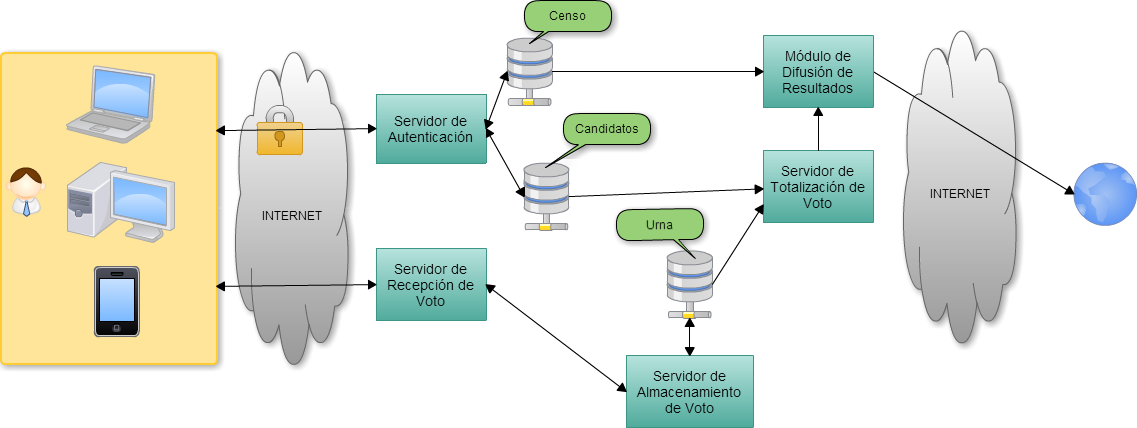
\includegraphics[width=1\textwidth]{imgs/sistema.png}
		\caption{Diagrama de flujo del Sistema}
		\label{fig:sistema}
	\end{figure}
	
	\begin{figure}[htbp]
		\centering
			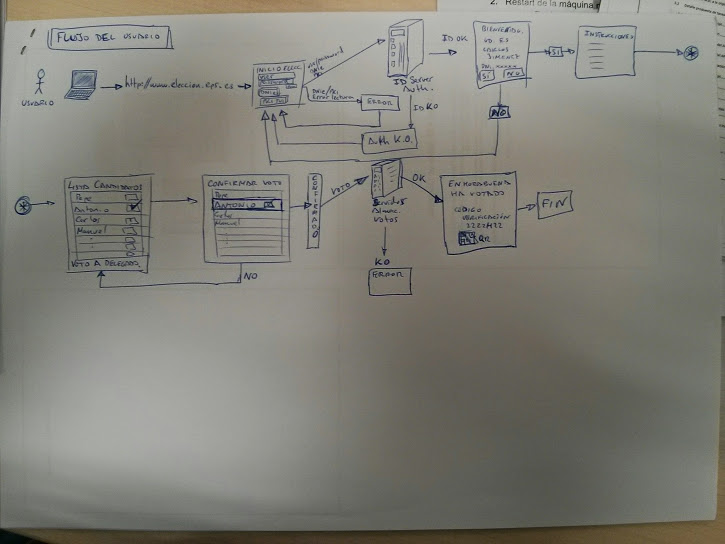
\includegraphics[width=0.60\textwidth]{imgs/flujoUsuario.jpg}
		\caption{Esquema del flujo que sigue el votante}
		\label{fig:flujoUsuario}
	\end{figure}
	\begin{figure}[htbp]
		\centering
			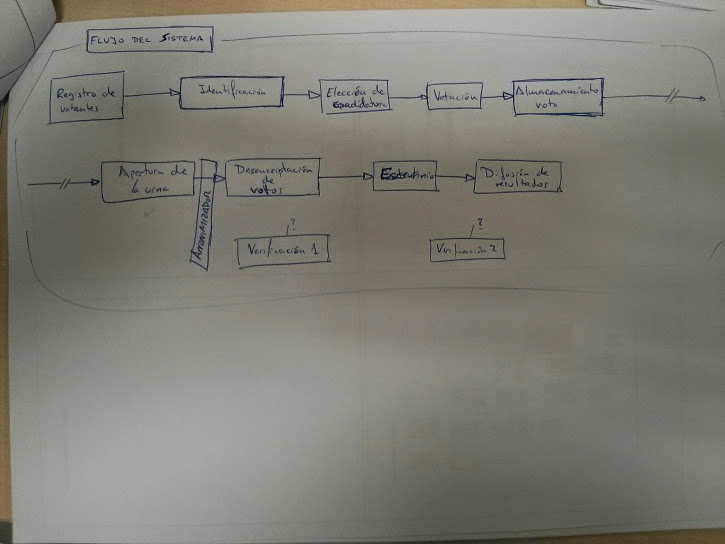
\includegraphics[width=0.60\textwidth]{imgs/flujoSistema.jpg}
		\caption{Esquema del flujo del Sistema}
		\label{fig:flujoSistema}
	\end{figure}
	
		
		\section{Dise�o}\label{dise�o}
			\subsection{Dise�o del esquema de votaci�n}\label{disenhoEsquemaVoto}
				\subsubsection{Registro}
				\subsubsection{Identificaci�n}
				\subsubsection{Elecci�n de candidatura}
				\subsubsection{Votaci�n}
				\subsubsection{Escrutinio}
				\subsubsection{Difusi�n de resultados}
				
			\subsection{Dise�o de la arquitectura}
			\subsection{Dise�o de la capa de datos}
			\subsection{Dise�o de la red}
			\subsection{Dise�o de la interfaz de usuario}\label{dise�o_interfaz_usuario}
				\subsubsection{Estructura de la p�gina web}
				\subsubsection{Estructura de la aplicaci�n m�vil}
				\subsubsection{Colores}
				\subsubsection{Logo de la elecci�n}
			
				\subsubsection{Ergonom�a}